\documentclass{standalone}

\usepackage{bm}
\usepackage{tikz}

\begin{document}
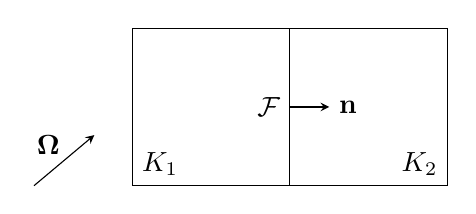
\begin{tikzpicture}[>=stealth]
	\draw (0,0) grid[step=2] (4,2); 
	\node[anchor=south west] at (0,0) {$K_1$}; 
	\node[anchor=south east] at (4,0) {$K_2$}; 
	\node[anchor=east] at (2,1) {$\mathcal{F}$}; 
	\draw[->] (2,1) -- (2.5,1) node[right] {$\boldsymbol{\mathrm{n}}$}; 
	\draw[->] (-1.25,0) -- node[midway, shift={(-.2,.2)}] {$\boldsymbol{\mathrm{\Omega}}$} +(40:1cm); 
\end{tikzpicture}
\end{document}